% Windows (DESIGN 4.3 item 1): steps that begin inside a figure, a
% TikZ picture, a minipage, an alignment, math, a loop's token lists and
% a \scantokens pseudo file. `scripts/ssa-edits --case windows` edits each.
\documentclass{article}
\usepackage{pgfplots}
\pgfplotsset{compat=1.18}
\begin{document}
\section{Windows}\label{sec:one}
Para1 This paragraph comes first, with a few words of text to make a line
or two of output. It refers to Figure~\ref{fig:plot} and to
Section~\ref{sec:one}.

Para2 A paragraph before the figure.\footnote{Foot1 A footnote, edited
later.}

\begin{figure}[ht]
  \centering
  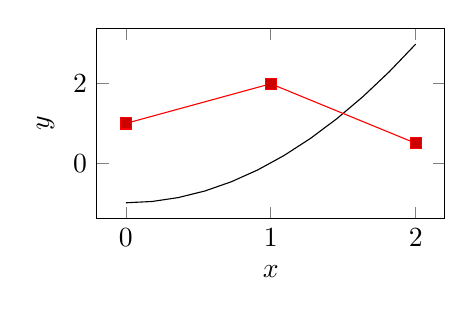
\begin{tikzpicture}
    \begin{axis}[width=6cm, height=4cm, xlabel={$x$}, ylabel={$y$}]
      \addplot[domain=0:2, samples=12] {x^2 - 1};
      \addplot coordinates {(0,1) (1,2) (2,0.5)};
    \end{axis}
  \end{tikzpicture}
  \caption{Cap1 A plot of a parabola and a polyline.}\label{fig:plot}
\end{figure}

Para3 After the figure, a paragraph with \emph{emphasis} and
$a^2+b^2=c^2$ in line.
\[ \int_0^1 x^2\,dx = \frac13 \]
Para4 The display continues the paragraph.

\noindent\begin{minipage}{0.5\textwidth}
Mini1 A paragraph inside a minipage, long enough to wrap onto a second
line of text.

Mini2 A second paragraph in the minipage.
\end{minipage}

\begin{tabular}{lr}
Cell1 & 1 \\
Cell2 & 2 \\
\end{tabular}

\newcount\n \n=0
\loop\advance\n by 1 Loop\the\n\ \ifnum\n<20 \repeat

\scantokens{Scan1 Rescanned text.}

Para5 The last paragraph.
\end{document}
